%-------------------------------------------------------------------------------
%                            BAB III
%               		METODOLOGI PENELITIAN
%-------------------------------------------------------------------------------
\fancyhf{} 
\fancyfoot[C]{\thepage}
\chapter{METODOLOGI PENELITIAN}

\section{Waktu dan Lokasi Penelitian}
Penelitian ini akan bertempat pada Gedung A Fakultas Matematika dan Ilmu Pengetahuan Alam. Waktu yang dibutuhkan agar penelitian ini dapat diimplementasikan adalah 4 bulan terhitung dari Juni 2022 hingga September 2022.

\section{Alat dan Bahan}
Alat dan bahan yang digunakan pada penelitian ini meliputi perangkat keras, perangkat lunak, dan data. Perangkat lunak yang digunakan dalam penelitian ini adalah sebagai berikut:

\begin{itemize}
	\item Windows 10 64 bit
	\item Linux Ubuntu 20.04.1
	\item Kaldi
	\item Vosk-api
	\item Python 
	\item Visual Studio Code 1.50.1
	\item Google Form
	\item Freemake Audio Converter 1.1.9
	\item SRILM 1.7.3
\end{itemize}

\par Sedangkan perangkat keras yang digunakan pada penelitian ini adalah 1 unit Laptop Acer Aspire A514-52G dengan RAM 12 GB, \textit{Processor} Intel® Core™ i5-10210U @ 1.60 GHz (8 CPUs), 2.1GHz, Kartu grafis NVIDIA GeForce MX250 dan Harddisk 1 TB. 

\section{\textit{Roadmap} Penelitian}
\textit{Roadmap} pada penelitian ini merupakan diagram yang menggambarkan rangkaian beberapa penelitian yang memiliki kesinambungan dalam rentang waktu 2019 sampai dengan 2020 yang dibagi menjadi 2 fase. Fase pertama pada tahun 2019 memiliki dua fokus penelitian \textit{indoor localization} dengan menggunakan \textit{Bluetooth Low Energy} (BLE) dan menggunakan \textit{Wireless Local Area Network} (WLAN) dapat dilihat pada gambar \ref{fig:fase1}. Lalu pada fase kedua pada tahun 2020 lebih berfokus pada penelitian \textit{indoor localization} dengan menggunakan BLE dapat dilihat pada gambar \ref{fig:fase2}. Aplikasi Navigasi \textit{Indoor} dibangun untuk Fakultas MIPA, karena memiliki gedung yang cukup luas dan memiliki banyak sub Gedung yang dibagi menjadi 6 bagian dari Gedung A sampai Gedung F. Aplikasi ini dapat berjalan dan memberikan arahan pada pengguna di dalam ruangan. Salah satu bagian dari aplikasi Navigasi \textit{Indoor} ini adalah aplikasi \textit{route guidance} untuk pengguna tuna netra. Aplikasi \textit{route guidance} ini menggunakan \textit{voice recognition} sebagai penghubung untuk mempermudah bagi pengguna tuna netra agar dapat menjalankan aplikasi ini. Penelitian ini terletak pada fase 2 di tahun 2020 dengan topik utama yaitu Aplikasi Navigasi \textit{Indoor} dengan sub topik untuk pengguna tunanetra. Penelitian ini memiliki batasan berupa pembangunan model \textit{voice recognition} seperti yang ditunjukkan pada gambar \ref{fig:fase2} dengan kata dicetak tebal berwarna merah sebagai berikut.

\begin{figure}[H]
  \begin{adjustbox}{addcode={\begin{minipage}{\width}}{\caption{%
      \textit{Roadmap} Penelitian Fase 1
      }\label{fig:fase1}\end{minipage}},rotate=90,center} %label gambar simpen disetelah capt
      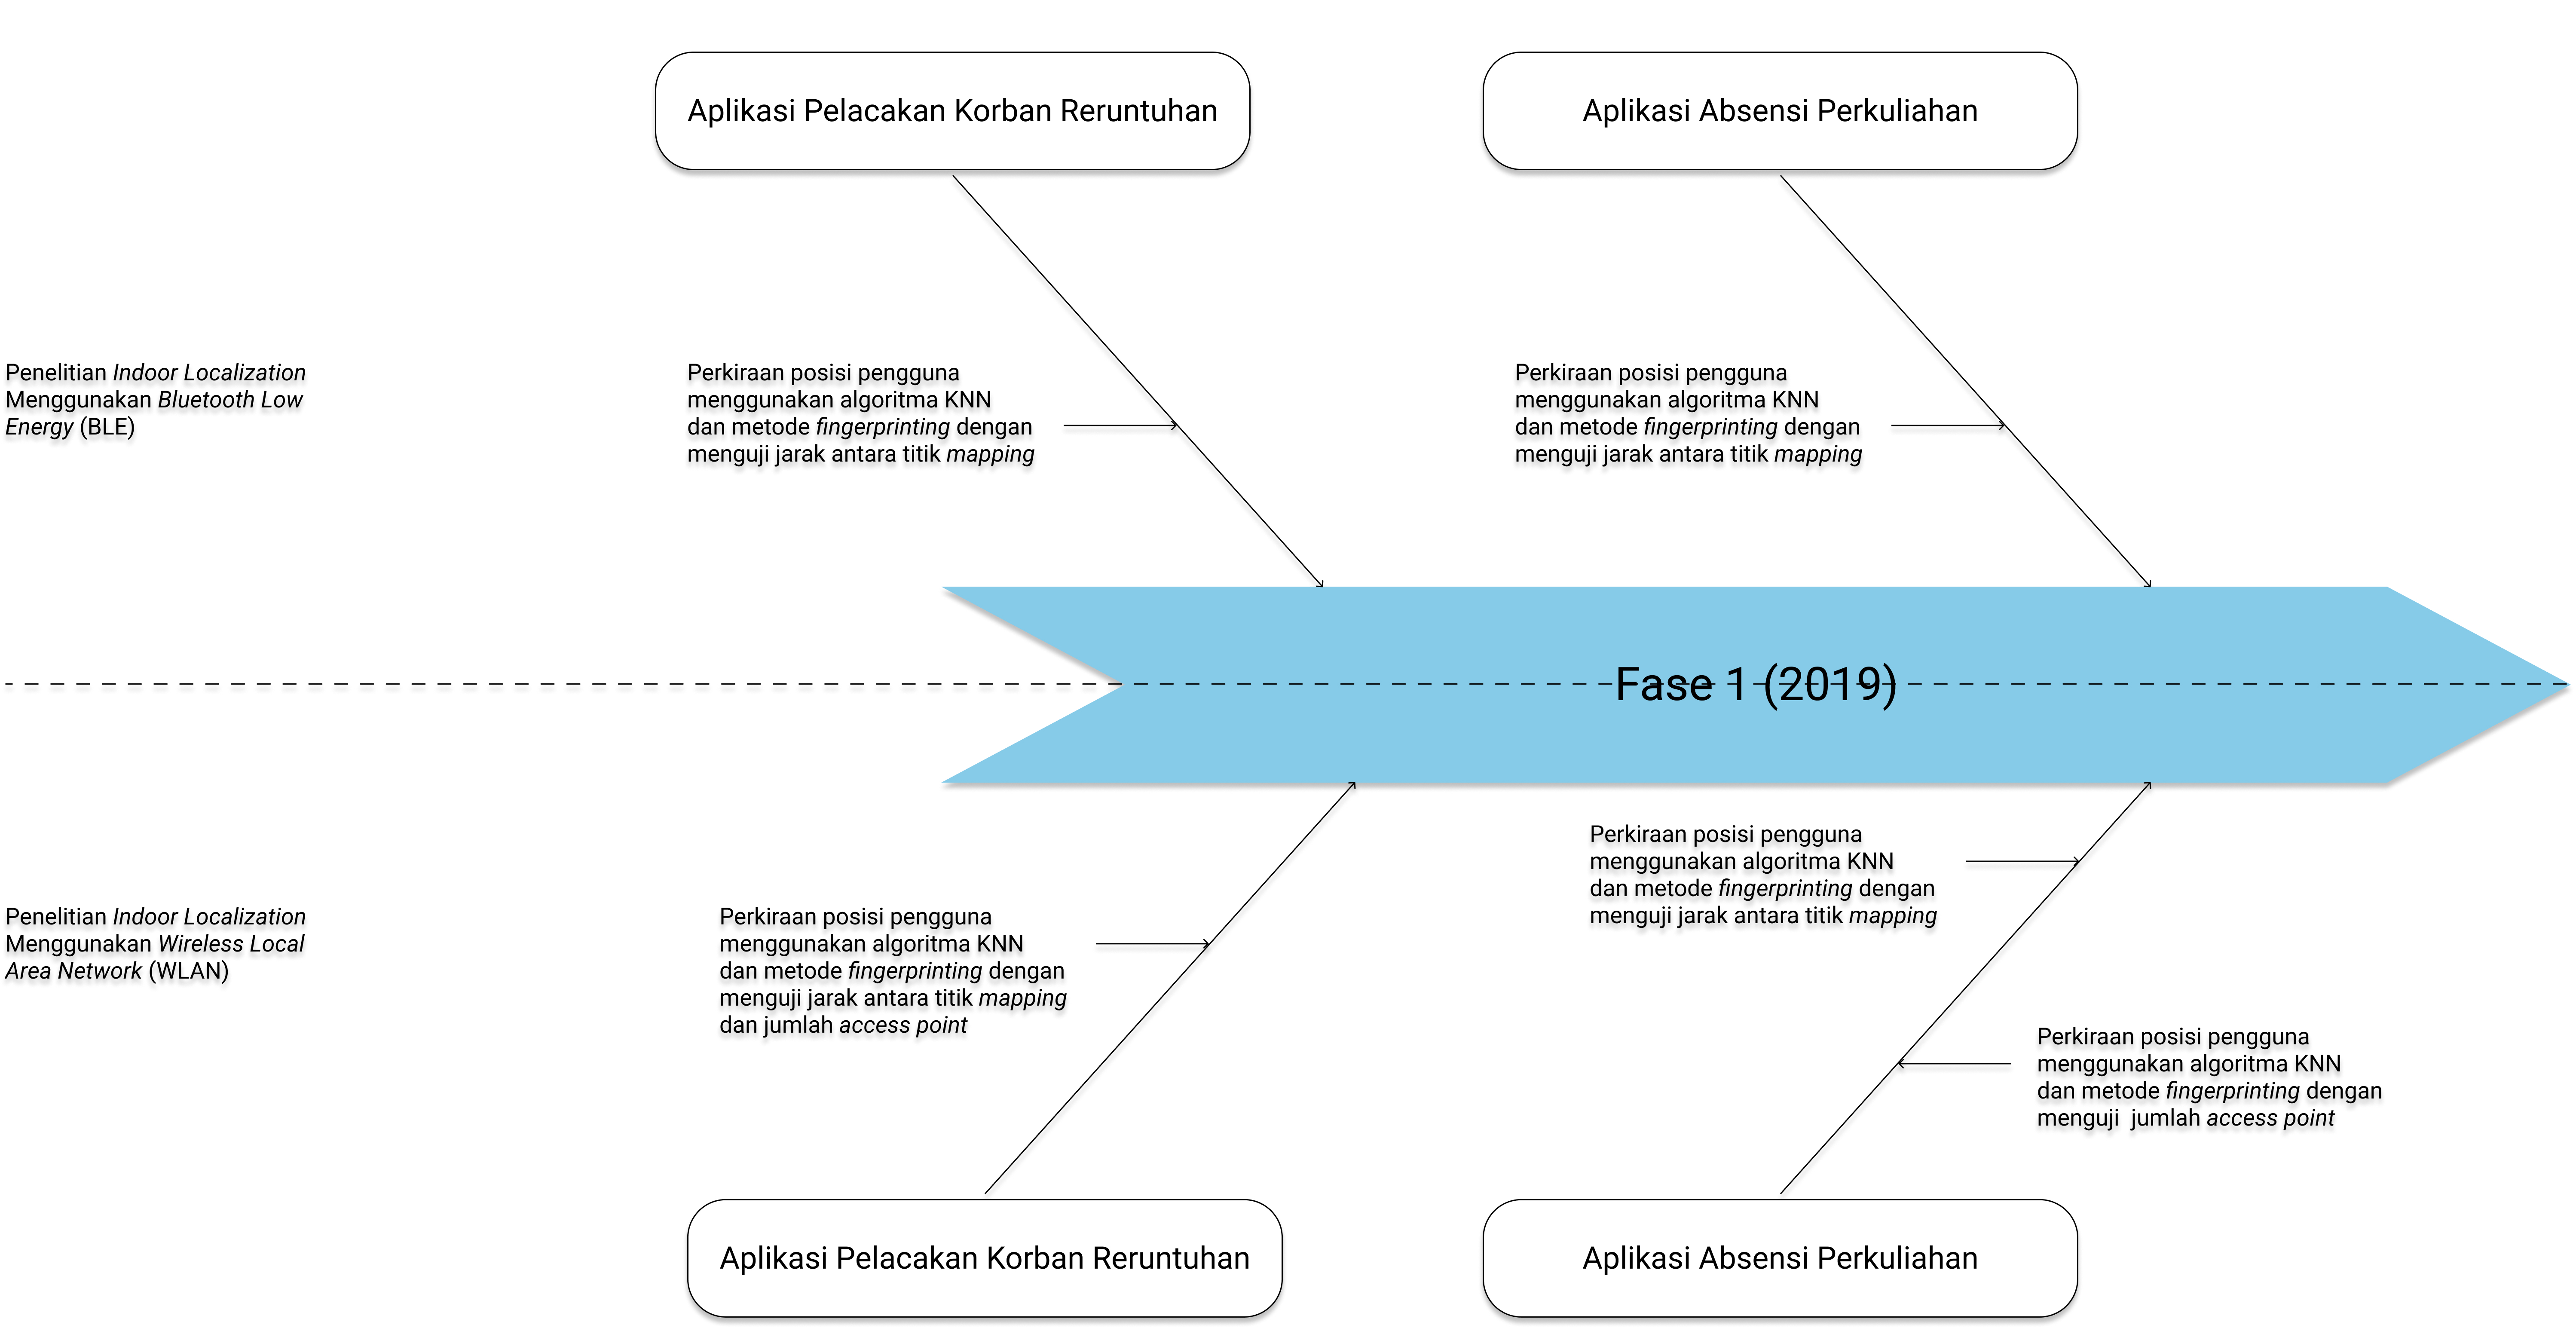
\includegraphics[scale=.3]{gambar/rp_fase1}%
  \end{adjustbox}
\end{figure}

\fancyhf{} 
\fancyfoot[R]{\thepage}

\begin{figure}[H]
  \begin{adjustbox}{addcode={\begin{minipage}{\width}}{\caption{%
      \textit{Roadmap} Penelitian Fase 2
      }\label{fig:fase2}\end{minipage}},rotate=90,center}
      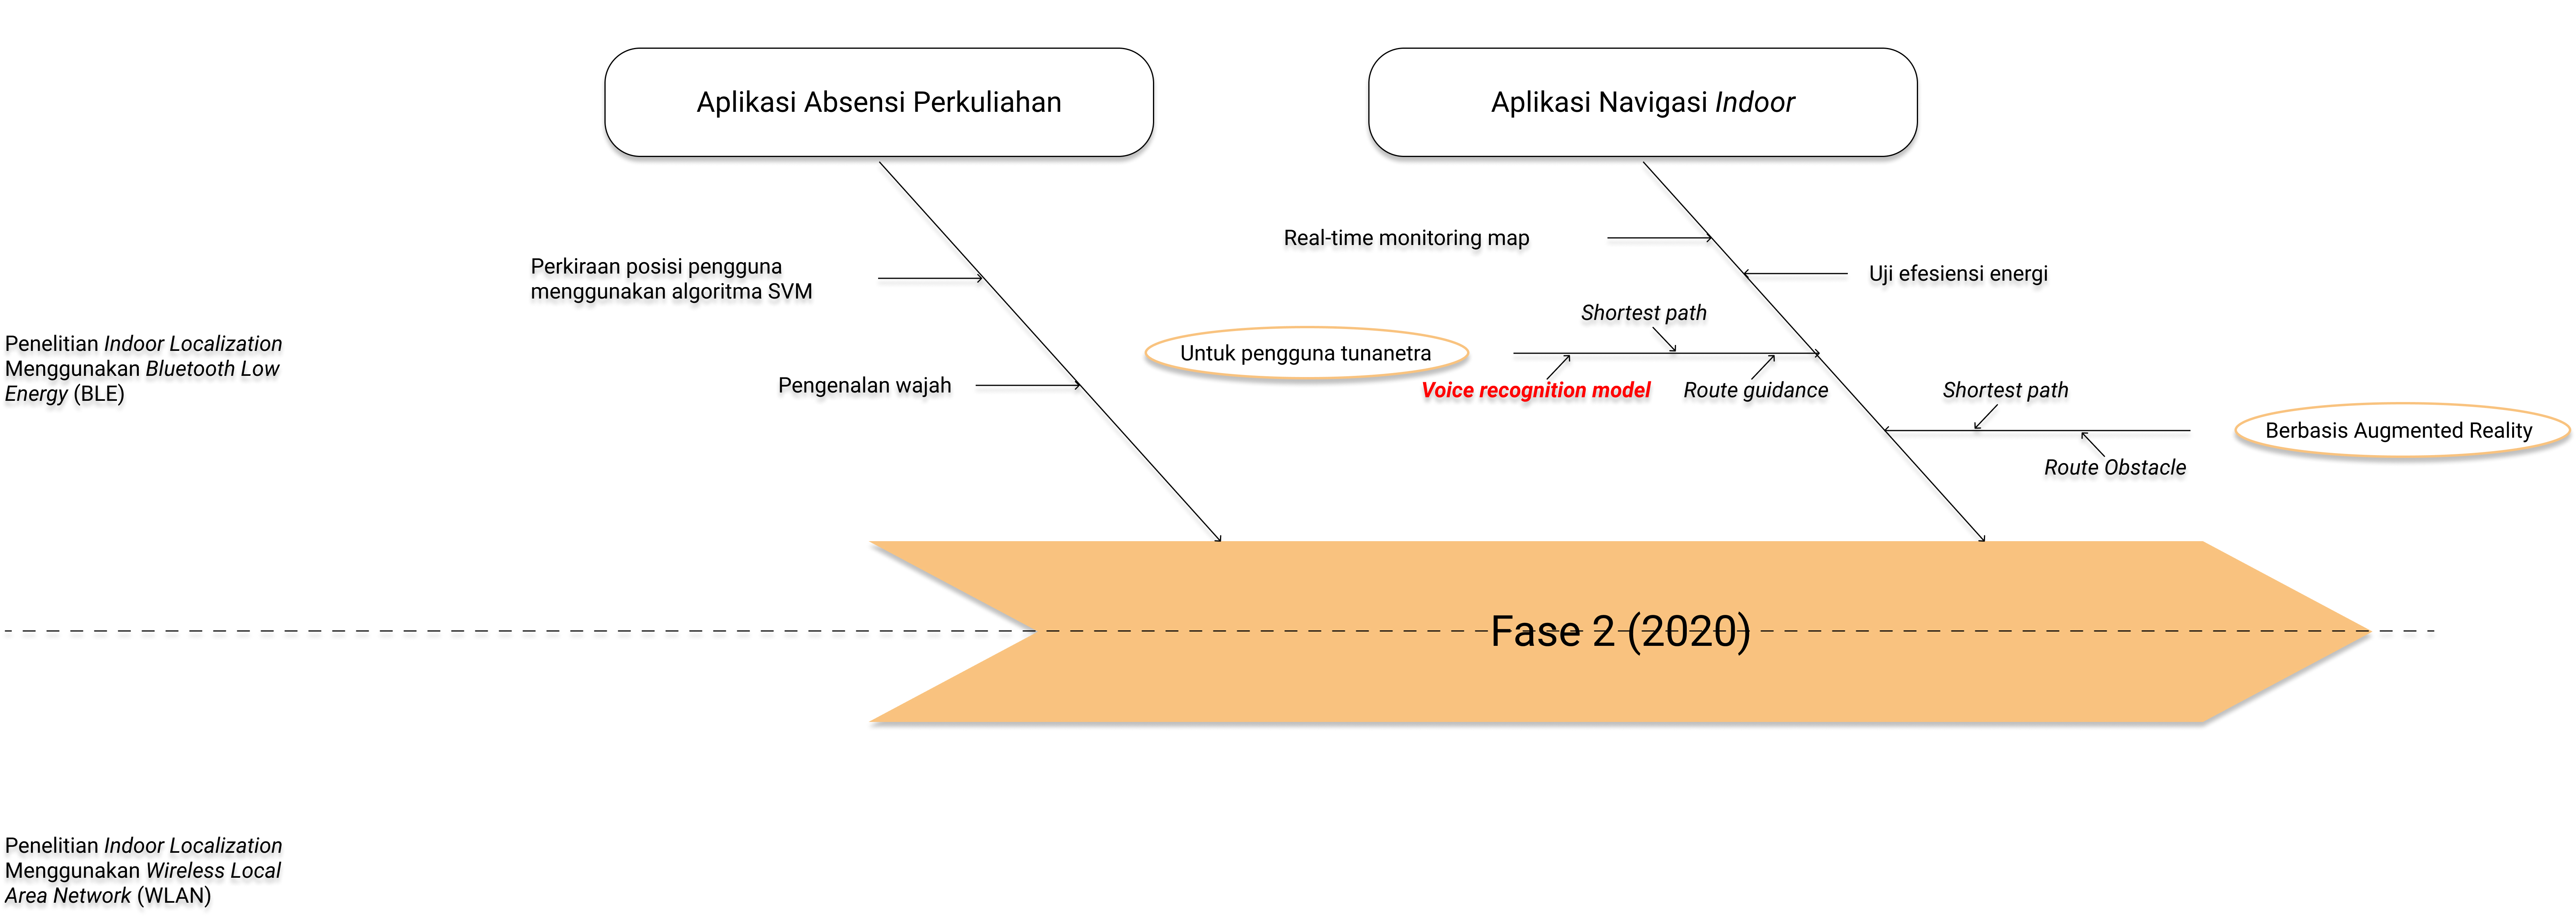
\includegraphics[scale=.3]{gambar/rp_fase2}%
  \end{adjustbox}
\end{figure}

\fancyhf{} 
\fancyfoot[R]{\thepage}

\section{Metode Penelitian}
Metode penelitian yang dilakukan dalam penelitian ini ditunjukkan pada Gambar \ref{sr_perancangan}.

\begin{figure}[H]
\centering
{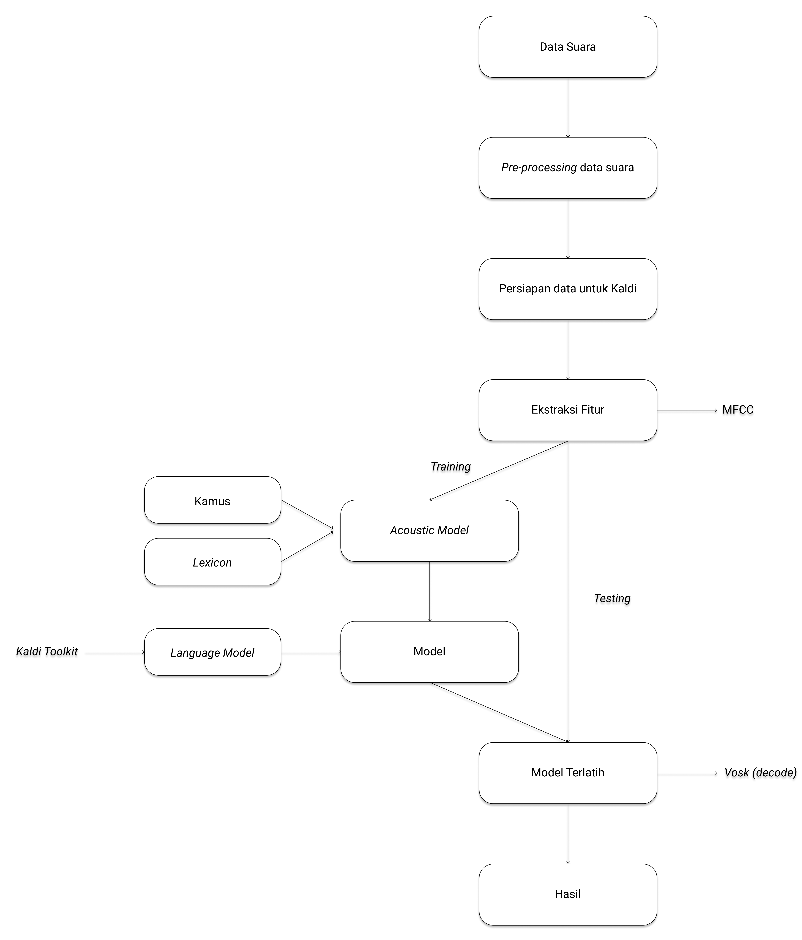
\includegraphics [width = 14cm, height= 16cm]{gambar/sr_perancangan}}
\caption{Diagram Perancangan Sistem Pengenalan Ucapan}
\label{sr_perancangan}
\end{figure}

\fancyhf{} 
\fancyfoot[R]{\thepage}

\subsection{Data Suara}
Pada tahap ini memiliki 2 hal yang dilakukan, yang pertama pembuatan transkrip dari nama-nama ruangan pada Gedung A FMIPA Unsyiah dan pengambilan data suara dari narasumber. Pada penulisan transkrip dilakukan dengan menggali informasi nama-nama ruangan pada Gedung A FMIPA dari beberapa orang. Setelah itu dilakukan proses pengambilan data suara oleh beberapa narasumber yang berjumlah 20 orang, memiliki rentang umur 17 tahun sampai dengan 58 tahun, memiliki 10 orang yang memiliki jenis kelamin laki-laki dan 10 orang memiliki jenis kelamin perempuan. Pengambilan suara dilakukan dengan 2 cara. Pertama melalui proses perekaman suara masing-masing melalui \textit{smartphone} masing-masing lalu di \textit{input} melalui \textit{form} yang sudah dibuat dengan Google Form. Kedua dilakukan perekaman suara dengan narasumber secara langsung tanpa melalui Google Form. Sebelum proses perekaman suara, narasumber diberikan 56 daftar nama-nama ruangan pada gedung A FMIPA Unsyiah serta diberi pengarahan dalam pengucapan dari daftar yang telah diberikan.

%%%%%%%%%%%%%%%%%%%%%%%%%%%%%%%%%%%%%%%%%%%
\subsection{\textit{Pre-processing} Data Suara}
Pada tahap ini dilakukan \textit{pre-processing} terhadap data suara yang sudah dimasukkan oleh narasumber. Tahap ini dilakukan karena narasumber melakukan proses perekaman suara secara mandiri dengan \textit{smartphone} masing-masing, jadi memiliki tipe \textit{file} audio yang berbeda-beda. \textit{File} audio diubah menjadi tipe \textit{file} *.wav dengan \textit{mono channel}, 16KHz \textit{sample rate} dan \textit{sample size} 16 bit. Aturan tersebut sesuai dengan yang diterima oleh Kaldi dan Vosk-api. Proses mengubah tipe file dengan menggunakan aplikasi Freemake Audio Converter, aplikasi ini dapat diinstalasi secara gratis dan dapat digunakan untuk sistem operasi Windows. 
Selain mengubah tipe \textit{file}, pada tahapan ini juga dilakukan pencocokan data berdasarkan nama-nama ruangan yang dikumpulkan menjadi satu \textit{folder}. Sehingga pada penelitian ini memiliki 20 \textit{folder} berbeda yang berisikan 56 \textit{file}. 56 \textit{file} tersebut merupakan jumlah narasumber atau yang dapat kita sebut di sini adalah \textit{speaker}.

%%%%%%%%%%%%%%%%%%%%%%%%%%%%%%%%%%%%%%%%%
\subsection{Persiapan Data untuk Kaldi}
Pada tahapan ini ada beberapa file yang harus disiapkan untuk membuat model \textit{speech recognition}, yaitu ada persiapan data akustik untuk membuat \textit{acoustic model} dan \textit{language data} untuk membuat \textit{language model}. Sebelum mempersiapkan beberapa \textit{file} yang dibutuhkan, data suara yang telah dikumpulkan di bagi menjadi 2 bagian, di mana 80\% \textit{speaker} untuk \textit{data training} dan 20\% speaker untuk \textit{data testing}. Berikut adalah penjelasan dari persiapan data akustik dan \textit{language data}:

\begin{enumerate}
\item Persiapan data akustik
\par Pada tahapan ini, ada 5 file yang harus dibuat agar Kaldi dapat memahami data audio yang akan diproses. Berikut adalah penjelasan file yang harus dibuat:
	\begin{itemize}
	\item Spk2gender
	\par Pada file ini berisikan informasi tentang nama yang diasumsikan sebagai \textit{id} dari \textit{speaker} dan jenis kelamin \textit{speaker} tersebut. \textit{File} ini memiliki \textit{pattern} <\textit{speakerID}> <jenis kelamin>, di mana jenis kelamin diinisialkan f sebagai perempuan dan m sebagai pria.
	
	\item Wav.scp
	\par Pada \textit{file} ini berisikan informasi \textit{utteranceID} dan lokasi audio tersebut ditambahkan dengan nama file tersebut, dalam hal ini penulisan \textit{utteranceID} merupakan \textit{speakerID} yang disambung dengan nama-nama ruangan yang diucapkan pada audio tersebut. Sehingga file ini memiliki \textit{pattern} <\textit{uterranceID}> <lokasi\_file\_audio>.	
	
	\item \textit{Text}
	\par Pada \textit{file} ini berisikan informasi tentang \textit{utteranceID} dan transkrip dari nama--nama ruangan di Gedung A FMIPA Unsyiah yang diucapkan oleh \textit{speaker}. Sehingga file ini memiliki \textit{pattern} <\textit{uterranceID}> <\textit{text\_transcription}>.
	
	\item Utt2spk
	\par Pada \textit{file} ini berisikan informasi berupa \textit{utteranceID} dan \textit{speakerID}, agar sistem pengenalan suara dapat mengetahui nama-nama ruangan yang diucapkan oleh \textit{speaker} tertentu. Sehingga file ini memiliki \textit{pattern} <\textit{uterranceID}> <\textit{speakerID}>.
	
	\item \textit{Corpus}
	\par Pada \textit{file} ini berisikan informasi berupa transkrip dari nama-nama ruangan di Gedung A FMIPA Unsyiah yang diucapkan oleh \textit{speaker}, namun \textit{file} ini disimpan pada lokasi yang berbeda dari beberapa \textit{file} yang sudah disebutkan sebelumnya. \textit{File} ini memiliki \textit{pattern} <\textit{text\_transcription}> yang ditulis per baris, sehingga \textit{file} pada penelitian ini terdapat 56 baris.
	\end{itemize}

\item Persiapan \textit{language data}
\par Pada tahapan ini, ada 4 \textit{file} berkaitan dengan \textit{language model}. Berikut adalah penjelasan \textit{file} yang harus dibuat:
	\begin{itemize}
	\item \textit{Lexicon}
	\par Pertama membuat \textit{file} yang bernama \textit{lexicon}.txt. Pada \textit{file} ini berisikan setiap kata dari \textit{dictionary} dengan penambahan \textit{phone transcriptions} atau penyebutan dari kata tersebut. Seperti contoh, jika ada kata `satu` maka penyebutan dari kata tersebut adalah sa tu. Namun, jika ada suara yang diam akan dideteksi sebagai \textit{silence phone} dan penyebutannya akan ditandai dengan `sil`. Sehingga file ini memiliki \textit{pattern} <\textit{word}> <\textit{phone} 1> <\textit{phone} 2>.
	
	\item \textit{Nonsilence phones}
	\par Lalu pada \textit{file} kedua diberi nama \textit{nonsilence\_phones}.txt. Pada \textit{file} ini berisikan \textit{list phone transcriptions} yang \textit{nonsilence phones}. Yang termasuk pada \textit{file} ini adalah semua \textit{phones} pada \textit{file lexicon} kecuali \textit{phones} seperti `sil` atau diam. \textit{File} ini memiliki \textit{pattern}: <\textit{phone}>.
	
	\item \textit{Silence phones}
	\par Pada \textit{file} ketiga diberi nama \textit{silence\_phones}.txt. Pada \textit{file} ini berisikan \textit{list phone transcription} yang diam atau `sil` pada bagian \textit{phone}. \textit{File} ini memiliki \textit{attern}: <\textit{phone}>.
	
	\item \textit{Optional silence}
	\par Pada \textit{file} keempat diberi nama \textit{optional\_silence}.txt. Pada \textit{file} ini berisikan \textit{list} pilihan lainnya dari \textit{silence phone transcription}. \textit{File} ini memiliki \textit{pattern}: <\textit{phone}>.
	\end{itemize}

\end{enumerate}

%%%%%%%%%%%%%%%%%%%%%%%%%%%%%%%%%%%%%%%%%

\subsection{Ekstraksi Fitur}
Setelah tahapan sebelumnya selesai dilakukan, selanjutnya masuk dalam tahapan ekstraksi fitur. Ekstraksi fitur dilakukan dengan menggunakan metode \textit{Mel Frequency Ceptral Coefficient} (MFCC), agar dapat mengidentifikasi konten linguistik dan membuang suara latar belakang serta suara yang tidak dibutuhkan dalam proses ini. Ekstraksi fitur pada penelitian ini memanfaatkan \textit{open source toolkit} untuk pengolahan suara yang tersedia yaitu Kaldi Toolkit. Pada perhitungan MFCC untuk penelitian ini ada hal yang harus ditentukan, yaitu menentukan jumlah \textit{ceptral coeffient} sebanyak 13 \textit{ceptral coeffient} dan jumlah \textit{frame} dalam suatu \textit{file} sepanjang 25 \textit{millisecond} dan memiliki \textit{window step} sebesar 10 \textit{millisecond}.

\subsection{Akustik Model}
Pada bagian ini merupakan tahapan untuk melakukan model akustik pada data training yang telah melewati proses ekstraksi fitur dengan MFCC. Tahapan ini menggunakan proses \textit{machine learning} dengan metode \textit{Deep Neural Network} (DNN) dan dilakukan juga pengambilan nilai \textit{CTC Loss} yang merepresentasikan akurasi dari \textit{training}. Pada tahap awal \textit{training} dimulai dengan menentukan jumlah \textit{file} yang masuk ke dalam perhitungan ke \textit{deep learning} sebagai bahan dari pembelajaran atau pembagi data. Setelah itu nilai dari MFCC \textit{feature} dimasukkan, lalu label untuk proses pembelajaran dimasukkan juga. Berikutnya dilakukan inisialisasi \textit{learning rate}, maksimal \textit{epoch} dan minimum \textit{loss} yang digunakan. Lalu pada proses perhitungan \textit{neural network} diinisialkan bobot yang dipakai. Selanjutnya metode \textit{deep learning} dengan \textit{input} nilai MFCC \textit{feature} dan target dihitung. Terakhir menampilkan nilai \textit{loss} dari hasil perhitungan yang didapat. Hal tersebut dilakukan sampai mendapatkan minimum nilai \textit{loss} dan maksimum nilai \textit{epoch}. Pada penelitian ini digunakan \textit{multilayer perseptron} sebagai layer pembelajarannya. 

\subsection{Model}
Setelah mendapatkan hasil dari \textit{acoustic modelling} dengan Kaldi, selanjutnya melakukan \textit{language modelling} dengan menggunakan SRILM (\textit{SRI Language Modeling Toolkit}). \textit{Language modelling} berguna agar dapat membedakan kata dan frasa yang terdengar serupa pada ucapannya sehingga didapatkan model pengenalan ucapan yang terlatih. 

\subsection{Model Terlatih}
Setelah model pengenalan ucapan sudah selesai dibangun, lalu model tersebut diletakan pada Vosk yang merupakan \textit{open source speech recognition toolkit}, Vosk dapat berjalan pada Android dengan API secara \textit{offline}. Data \textit{testing} yang sebelumnya sudah dipisahkan, diuji pada model tersebut sehingga mendapatkan keluaran berupa \textit{text}. Model ini akan dapat berjalan pada aplikasi Android \textit{route guidance} untuk tuna netra berbasis \textit{Indoor Positioning} yang akan dibangun.

%-----------------------------------------------------------------------------%

% Baris ini digunakan untuk membantu dalam melakukan sitasi
% Karena diapit dengan comment, maka baris ini akan diabaikan
% oleh compiler LaTeX.
\begin{comment}
\bibliography{daftar-pustaka}
\end{comment}